% Chapter 1

\chapter{Result} % Main chapter title

\label{Chapter2} % For referencing the chapter elsewhere, use \ref{Chapter1} 

%----------------------------------------------------------------------------------------

\section{Run1 (20170109-2017012; KEK)}
\subsection{Member}
Yuki, Cory, Bin-Hua, Takaaki, Takahiro
\subsection{Test setup}
\begin{figure}
	\begin{center}
                 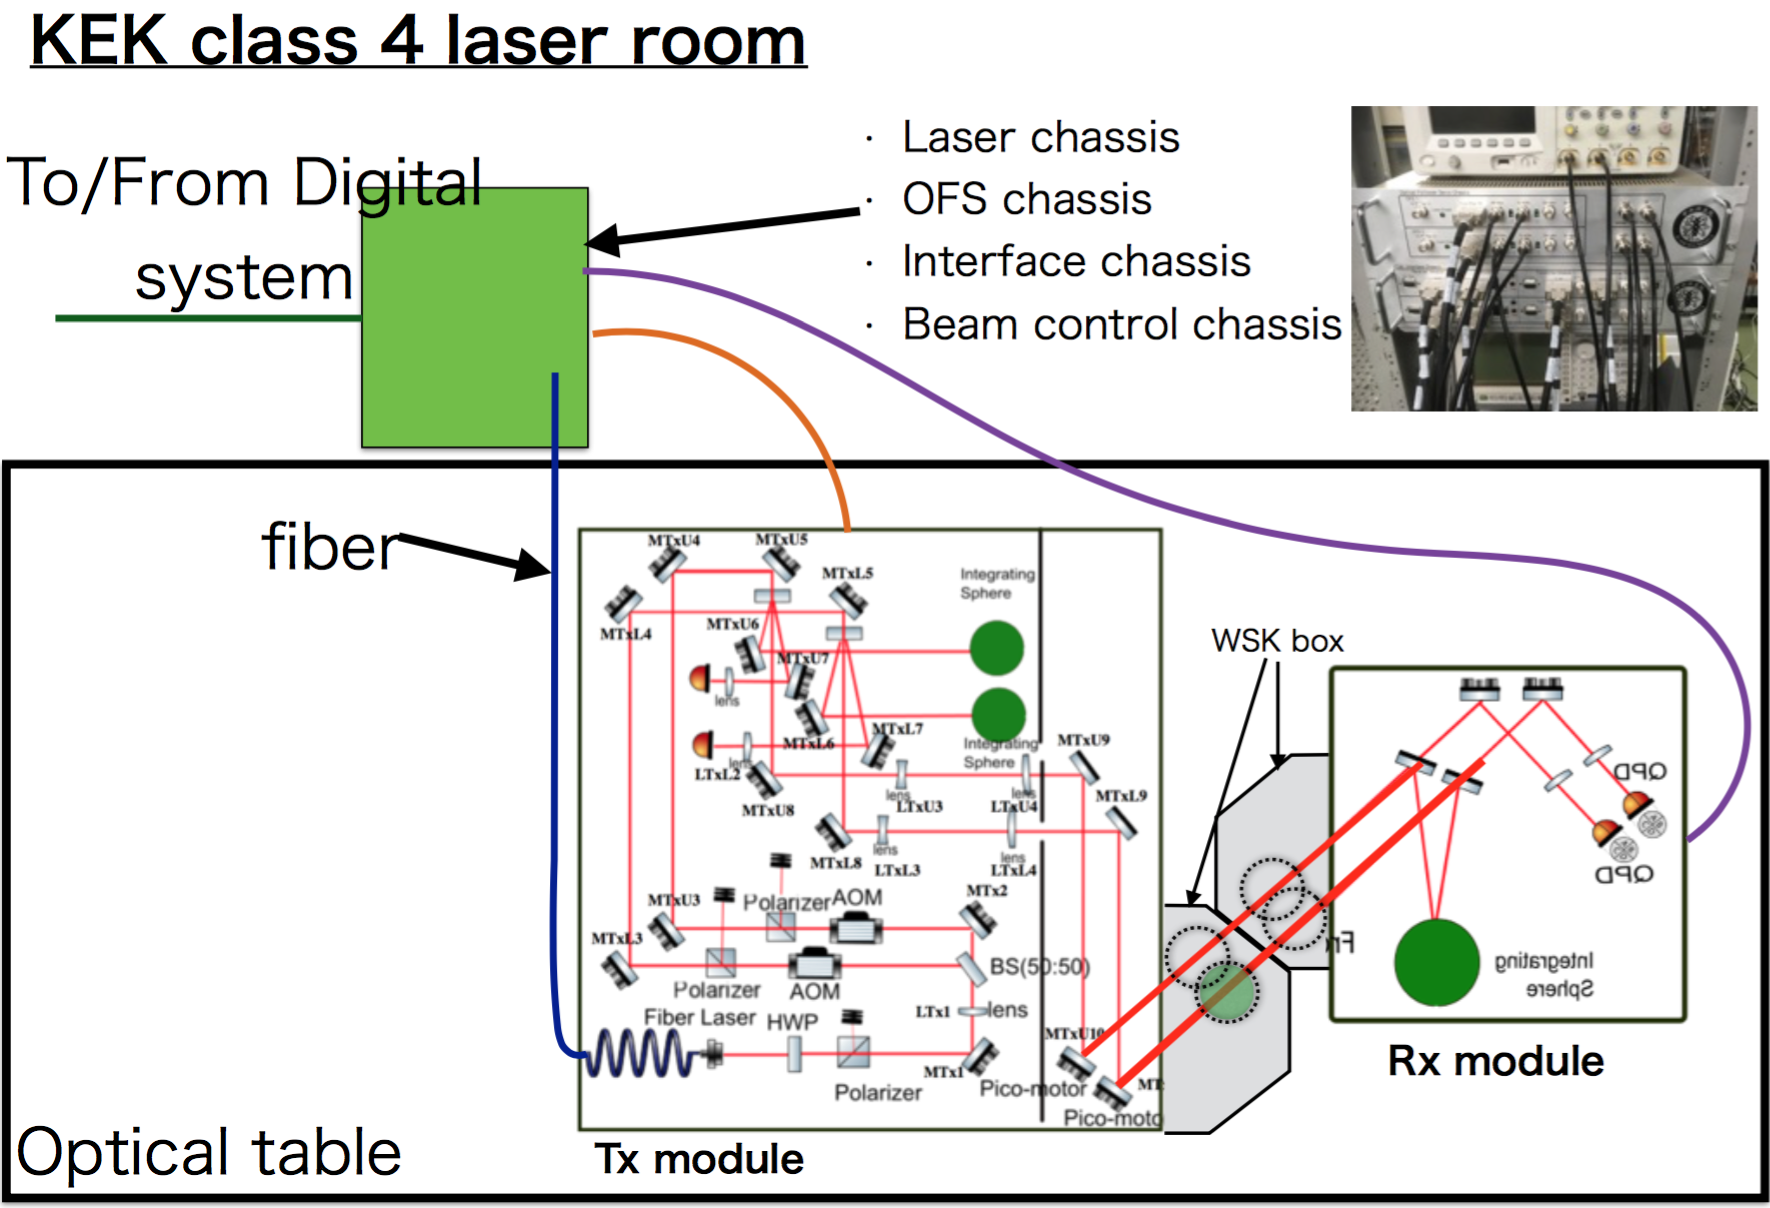
\includegraphics[width=15cm]{Setup_170109.eps}
                 \caption{Setup of the integration test} 
                 \label{fig:Setup} 
	\end{center}
\end{figure}
\begin{figure}
	\begin{center}
                 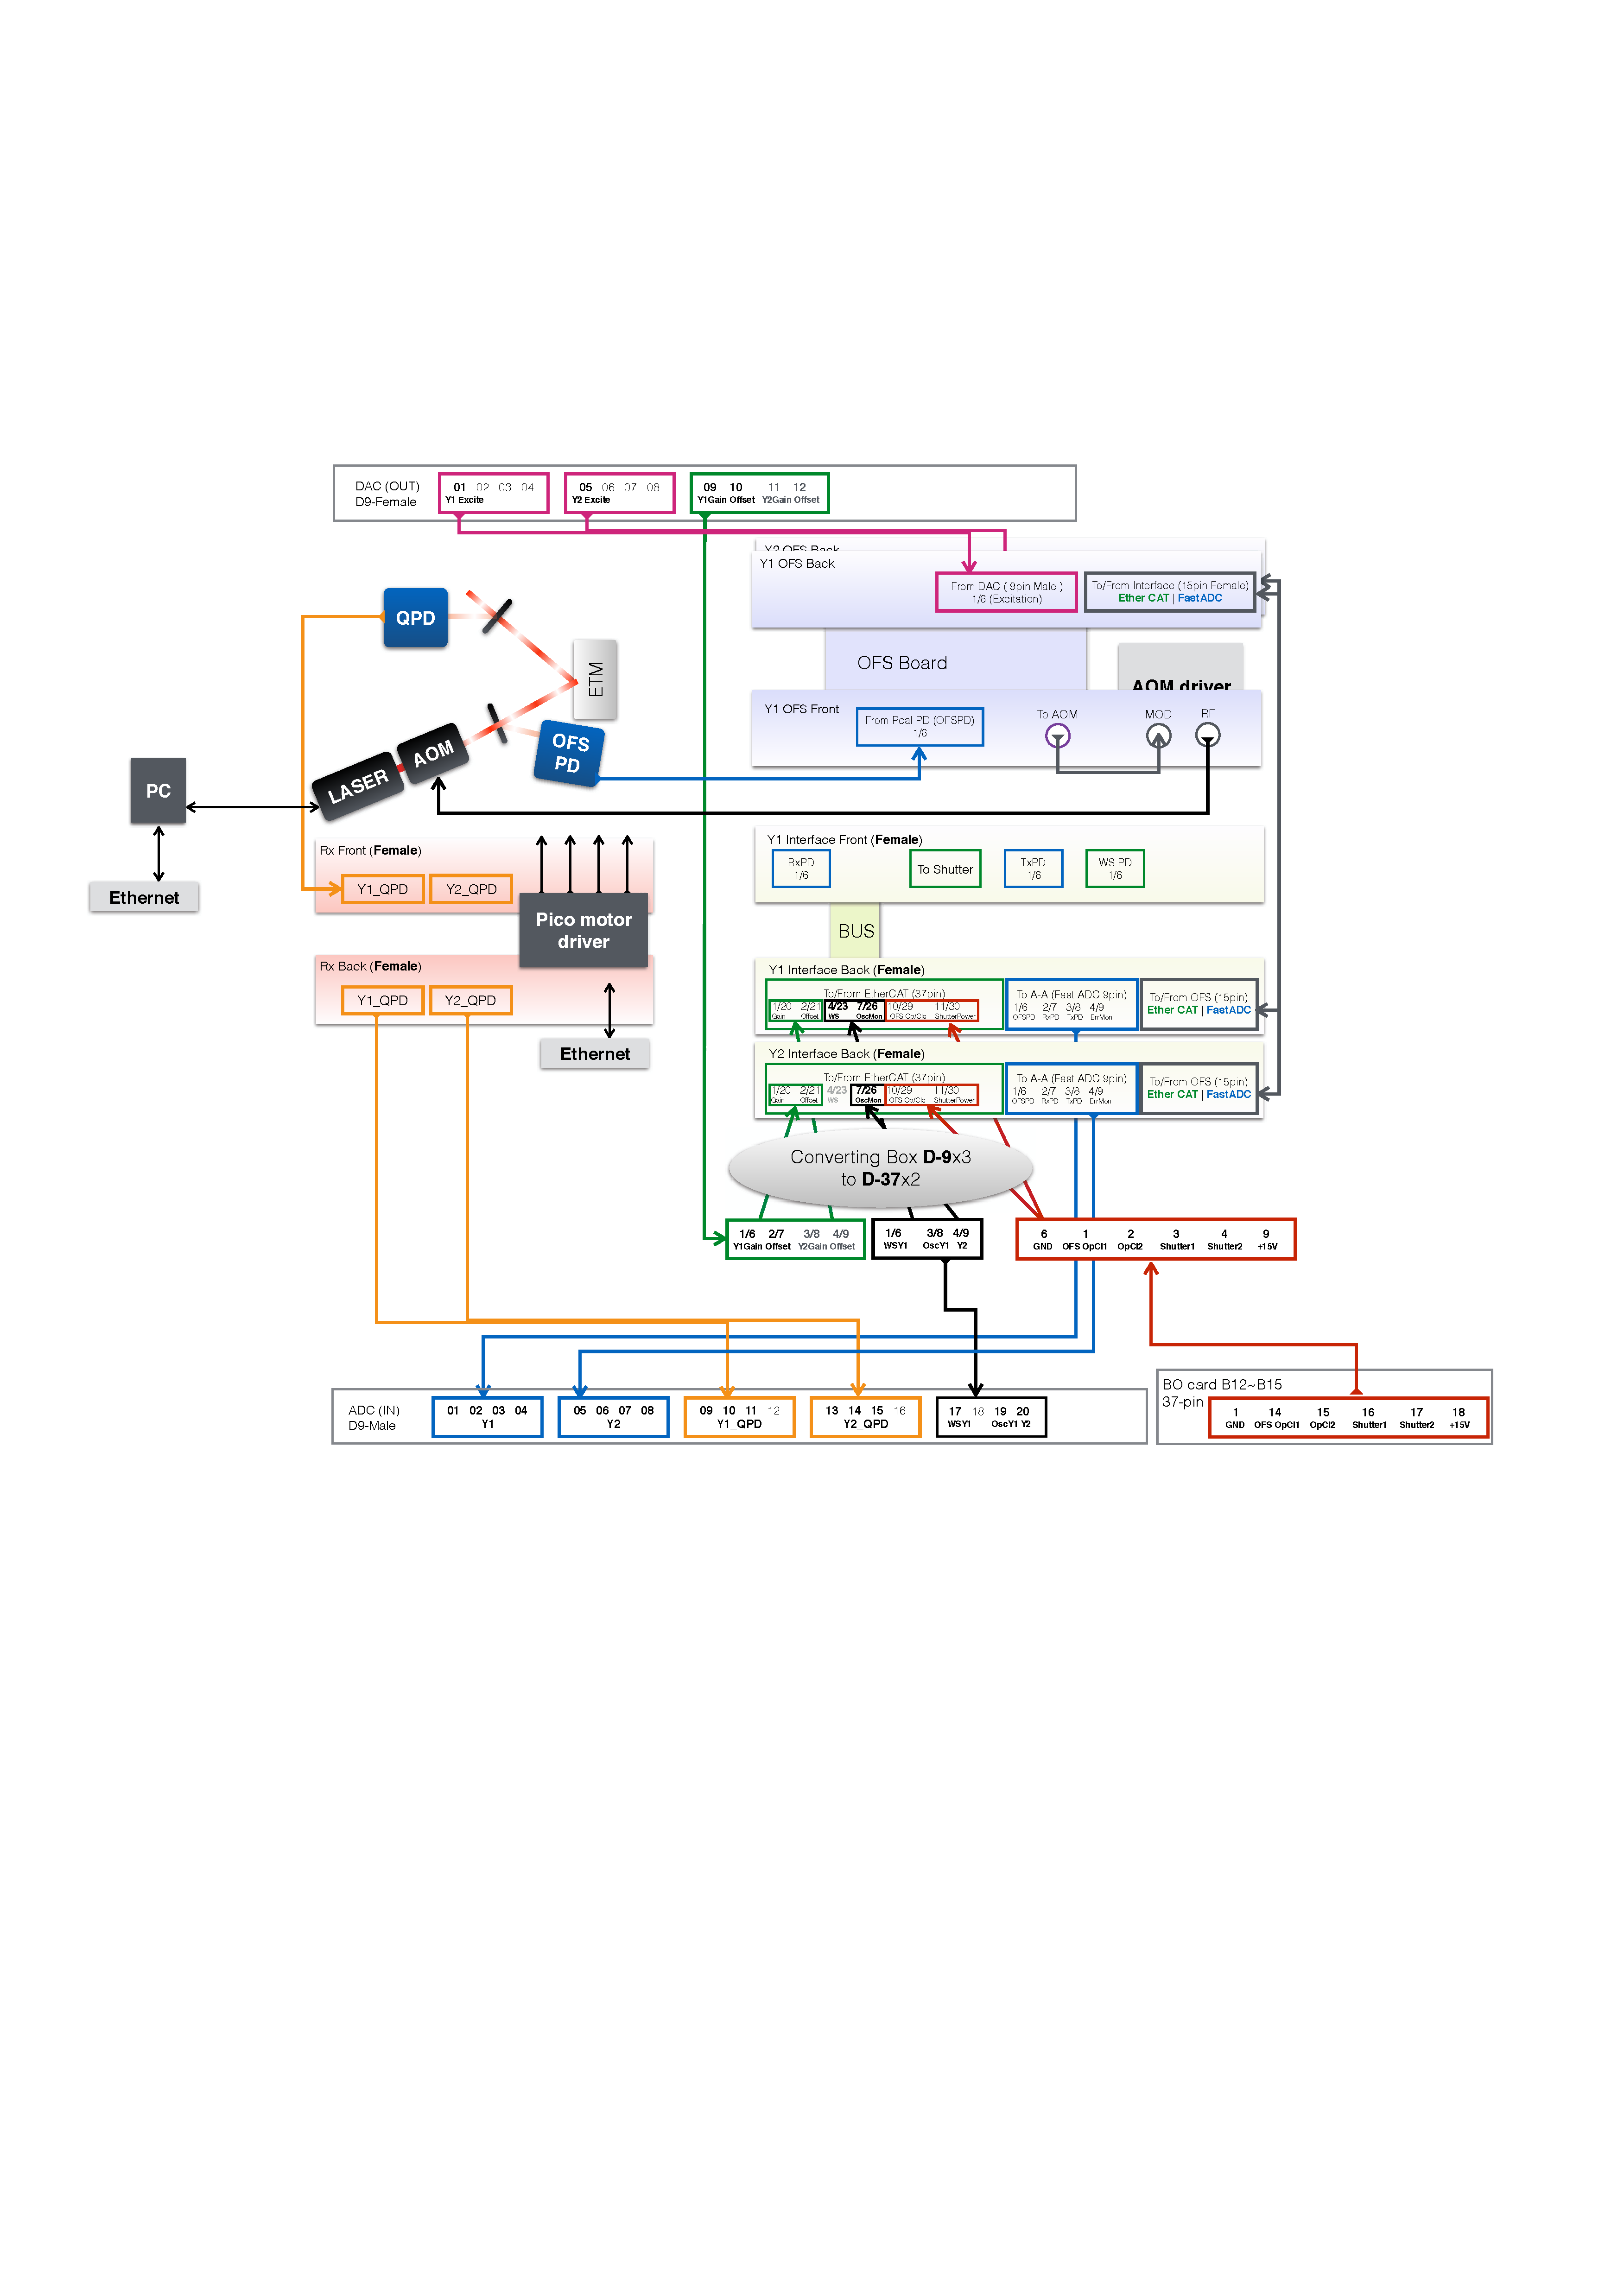
\includegraphics[width=18cm]{connection}
                 \caption{Setup of Control System for Integration Test} 
%                 \label{fig:Setup} 
	\end{center}
\end{figure}
\begin{figure}
	\begin{center}
                 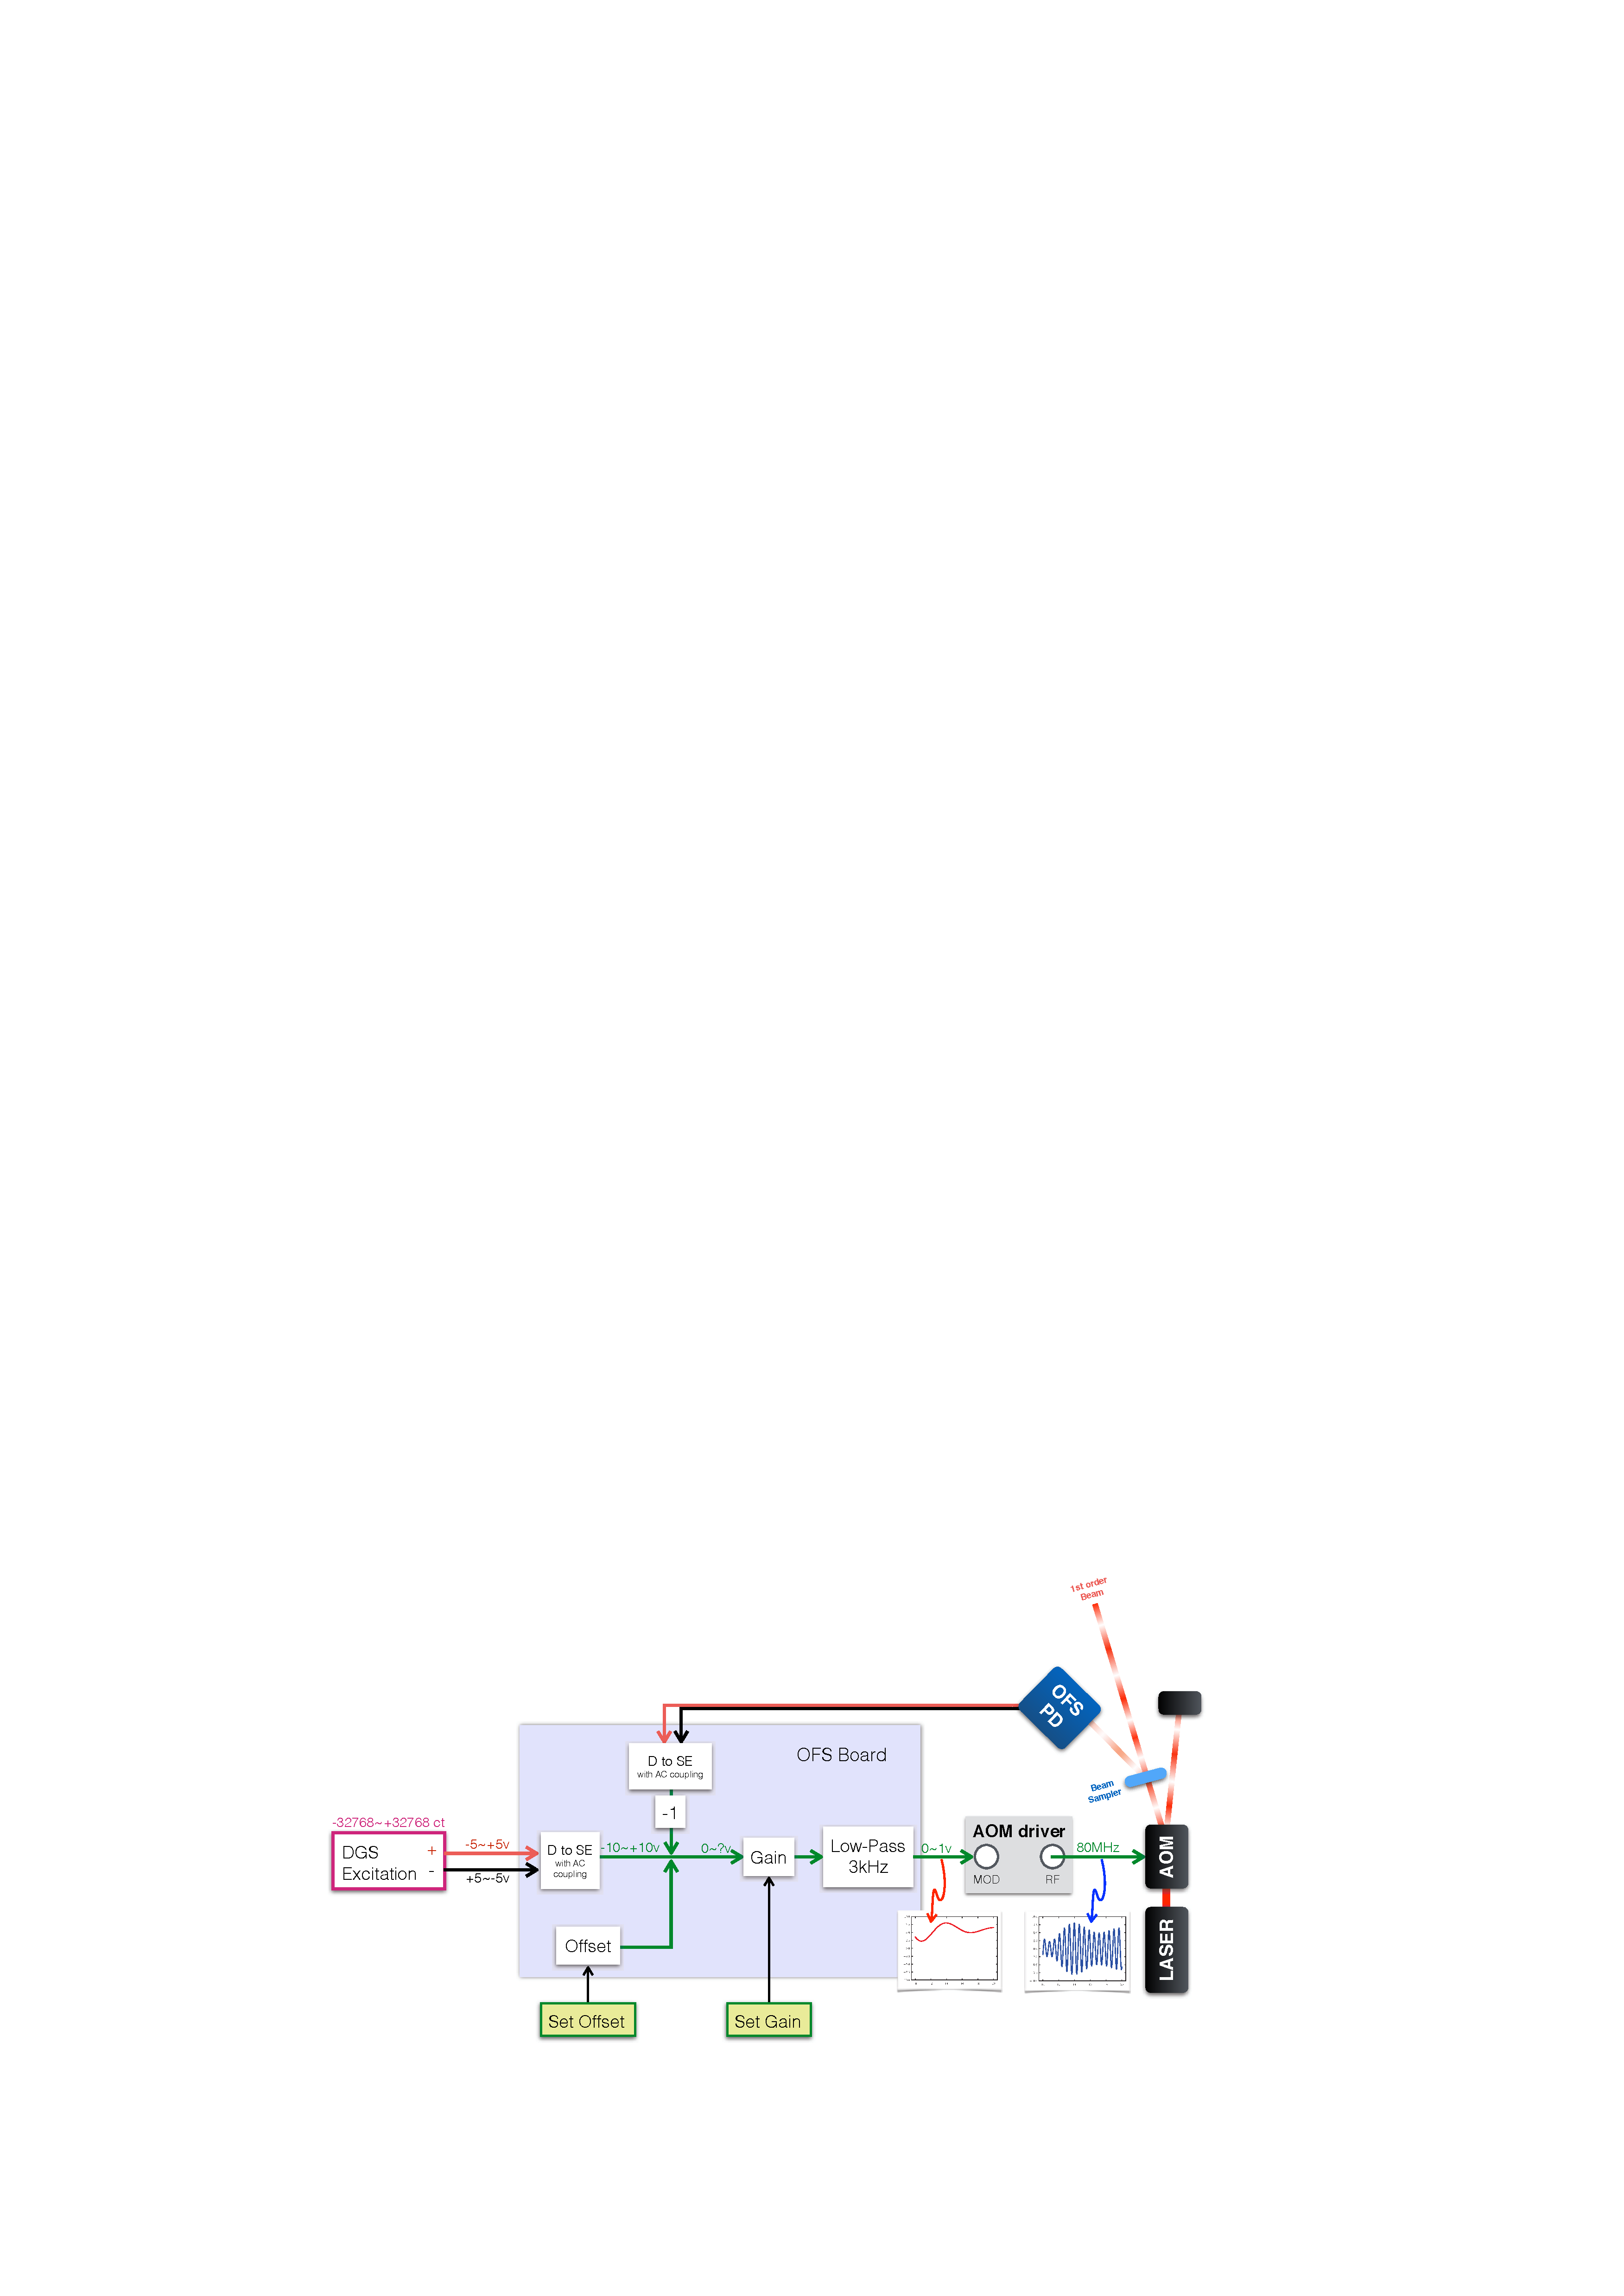
\includegraphics[width=15cm]{ofsPlot}
                 \caption{Block diagram of injecting signal through OFS board} 
%                 \label{fig:Set up} 
	\end{center}
\end{figure}
\pagebreak
\subsection{Log: 01\/09}
Main goal of Jan. 9th measurement is noise debugging.
In previous measurement, the measured noise is larger than that of requirement.
To reduce the noise, we tried the following things:
\paragraph{Open loop gain}


\pagebreak

\subsection{Injection Test}
\subsubsection{Time delay measurement}

To investigate the time delay of PCal system, we injected some Sine-Gaussian signal.
 Sine-Gaussian signal for our injection test is defined as Eq.~\ref{eq:singaussian}
\begin{equation}
\label{eq:singaussian}
    A \exp\left(-\frac{(t-t_0)^2}{\tau^2}\right) \cos ( 2 \pi f_0 (t-t_0))
\end{equation}
\begin{equation*}
   \tau = \frac{Q}{ \sqrt{2} \pi f_0}
\end{equation*}



\noindent
First, We directly connect the Digital System "Excitation" port and OFS\_PD port for measuring time delay caused by Digital System itself, the result is summarized in Table~\ref{tab:timedelayDGS}.
\begin{table}[htbp]
   \centering
   %\topcaption{Table captions are better up top} % requires the topcapt package
   \begin{tabular}{ ccrcc } % Column formatting, @{} suppresses leading/trailing space
      \toprule
%      \multicolumn{2}{c}{Item} \\
                 &    &  & DAC 1\_0              & ADC 1\_0  \\

     \cmidrule(r){3-5} % Partial rule. (r) trims the line a little bit on the right; (l) & (lr) also possible
      $f_0$ (Hz) &    &  & DAC 1\_0 GPS Time (s) & ADC 1\_0 delayed Time (s) \\
      \midrule
        35  &    &    &   &\\
        330 &    &    &   &\\
        1k  &    &    &   &\\
        3k  &    &    &   &\\
      \bottomrule
   \end{tabular}
   \caption{Time delay measurement results of Digital System, $A=$1V, $Q=$20 }
   \label{tab:timedelayDGS}
\end{table}

\noindent
Then, We connect "Excitation" port to OFS board and OFS\_PD port to Interface Chassis for measuring time delay between excitation and OFS\_PD, which are corresponding to the input and output of Optical Follower Servo. See Table~\ref{tab:timedelay}.

% Requires the booktabs if the memoir class is not being used
\begin{table}[htbp]
   \centering
   %\topcaption{Table captions are better up top} % requires the topcapt package
   \begin{tabular}{ ccrcc } % Column formatting, @{} suppresses leading/trailing space
      \toprule
%      \multicolumn{2}{c}{Item} \\
%      \cmidrule(r){1-2} % Partial rule. (r) trims the line a little bit on the right; (l) & (lr) also possible
       $f_0$ (Hz) &    & & Injected GPS Time (s) & OFS\_PD GPS Time (s) \\
      \midrule
        35  &    &    &   &\\
        330 &    &    &   &\\
        1k  &    &    &   &\\
        3k  &    &    &   &\\
      \bottomrule
   \end{tabular}
   \caption{Time delay measurement results of PCal, $A=$1V, $Q=$20}
   \label{tab:timedelay}
\end{table}




\pagebreak
\subsubsection{CBC Injection Test}

%\begin{equation}
%\label{eq:pcaleq}
%    \Delta L (f) (\mathrm{m} / \mathrm{Hz}) = \frac{2 \Delta P \cos(\theta)}{c} \frac{1}{M (2 \pi f )^2}
%\end{equation}

\begin{align}
%\label{eq:pcaleq}
    \frac{F(t)}{M}=\frac{1}{M} \frac{2 P(t) \cos(\theta)}{c} &= \ddot{x}(t)
\end{align}

For $x=x_0 \sin(\omega t)$,
\begin{align}
%\label{eq:pcaleq}
    \frac{1}{M} \frac{2 P_0 \cos(\theta)}{c} \sin(\omega t) &=  -\omega^2 x_0 \sin(\omega t)
\end{align}

Thus,
\begin{align}
%\label{eq:pcaleq}
    P_0 &= -\omega^2 \frac{M c}{2 \cos(\theta)} x_0 = -\omega^2 \frac{M c}{2 \cos(\theta)} L h_0
\end{align}
\begin{align*}
%\label{eq:pcaleq}
    M &= 23 ~\mathrm{kg} \\
    L &= 3 ~\mathrm{km}  \\
    \theta &= 0.72 ~\mathrm{deg}  \\
    c &= 2.998\times10^8 ~\mathrm{m/s} \\
    P_0 ~(\mathrm{Watts}) \times Gain_{\text{~Power to OFSPD}} &= 
     \underbrace{V_{\text{OFSPD}}}_{\text{Same as V$_{\text{Injection}}$}}~ (\mathrm{Volts}) \\
\end{align*}
Therefore, the overall gain should be set in injection channel, which is in Volt unit, is
\begin{align}
%\label{eq:pcaleq}
    \omega^2 \frac{M c}{2 \cos(\theta)} L \times Gain_{\text{~Power to OFSPD}} 
\end{align}

\pagebreak

\section{Run2 (201702; Toyama)}

\section{Run3 (201703; KAGRA Y-end)}
%----------------------------------------------------------------------------------------

